% This is samplepaper.tex, a sample chapter demonstrating the
% LLNCS macro package for Springer Computer Science proceedings;
% Version 2.20 of 2017/10/04
%
\documentclass[runningheads]{llncs}
%
\usepackage{graphicx}
\usepackage{subcaption}
\usepackage{float}
\usepackage{todonotes}
\usepackage{amsmath}
% Used for displaying a sample figure. If possible, figure files should
% be included in EPS format.
%
% If you use the hyperref package, please uncomment the following line
% to display URLs in blue roman font according to Springer's eBook style:
% \renewcommand\UrlFont{\color{blue}\rmfamily}

\begin{document}
%
\title{Embedded Reachability for Half the Price\thanks{Supported by organization x.}}
%
%\titlerunning{Abbreviated paper title}
% If the paper title is too long for the running head, you can set
% an abbreviated paper title here
%
\author{Nathan Jewell\inst{1}\orcidID{0000-1111-2222-3333} \and
Stanley Bak\inst{2}\orcidID{2222--3333-4444-5555} \and
Houssam Abbas\inst{1}\orcidID{1111-2222-3333-4444}} 
%
\authorrunning{N. Jewell et al.}
% First names are abbreviated in the running head.
% If there are more than two authors, 'et al.' is used.
%
\institute{Oregon State University, Corvallis OR 97333, USA \and
\email{jewelln@oregonstate.edu}}
\institute{Stony Brook University, USA \and
\email{jewelln@oregonstate.edu}}
%
\maketitle              % typeset the header of the contribution
%
\begin{abstract}
Reachability analysis enables the safety assurance of control systems despite uncertain initial conditions and control inputs, and can be an important component to run on-board an autonomous system.
This tool paper demonstrates that it is possible to obtain accurate, real-time reachability computations for an autonomous vehicle using only simple kinematics, parallelization on a GPU without algorithmic changes, and while running a full autonomous racing stack.
%This stands in contrast to existing work which required the development of custom parallelizable reachability algorithms, the use of accurate nonlinear models of the dynamics, and was limited to a shorter look-ahead horizon. 
We leverage HYLAA, a state-of-the-art reachability tool.
Our solution uses simple linearized kinematics, yet it is accurate; runs in Python, yet is real-time; shares the hardware with a full autonomous racing stack including a state-of-the-art optimization-based predictive controller; and is partitioned between CPU and GPU using only code-level parallelization.
In our testing we achieve accurate 10-step reachability as quickly as 150 milliseconds. 
We also find that porting portions of reachability onto the GPU can improve the runtime for 10-step reachability by 62\% over a CPU only implementation.% and reduces the computational complexity in relation to number of reachability steps.
We demonstrate our results on the F1/10 1/10th-scale autonomous race car.
This work lowers the barrier to running reachability significantly, as it reduces the need to do time-consuming system identification, the need to employ nonlinear reachability tools, and the need to do algorithmic modifications to enable GPU parallelization.

\keywords{Reachability  \and Safety Analysis \and CUDA \and GPU}
\end{abstract}
%
%
%
\section{Introduction}
Reachability is the computation of possible future system states, given a set of initial states and a set of possible inputs at each time step. 
In discrete-time reachability, a range of $N$ reach sets are computed for $N$ future times $dt$, $2dt$,..., $Ndt$, with the guarantee that any state actually reached at time $idt$ is within the $i^{th}$ computed reach set; thus the latter can be utilized for safety analysis\cite{malerintro}.
Specifically, with safety-critical systems, it is necessary to verify that no error state could be reached. In autonomous vehicles, error states may involve intersections with walls, other cars or people, etc.. By checking that the reach set does not contain error states, a guarantee is obtained that the next $N$ time steps are safe.  
Planned inputs can then be modified to avoid danger, preventing potentially catastrophic system failure. 

In this work we set out to see whether it is possible to obtain accurate and timely reachability computations using a common CPU+GPU hardware on-board an autonomous vehicle, with minimal upfront effort, and while running an entire autonomous driving stack.
Minimal effort means no system identification, no tuning of parameters, no algorithmic modifications, etc. 
While this seems to go against the desire to have guaranteed computations, it has the advantage of significantly lowering the barrier to running reachability analysis, and we show empirically that the computations are still accurate. GPU based implementations of reachability include, Xspeed which introduces algorithms optimized for GPU performance. \cite{xspeed}.
%We explore a number of different runtime modes for profiling reachability computation. These modes are chosen to stress different components of the host system, improve runtime, and demonstrate the impact of a functional autonomous navigation stack on performance.

\section{Background}
\subsection{F1/10 Platform}
Our experiments used the F1/10 autonomous racing platform which is a standardized hardware platform designed to facilitate algorithmic improvements for high-reliability autonomous systems. The vehicle consists of a modified one tenth scale remote control car chassis and is equipped with an improved electronic speed controller and LIDAR. The compute platform is an NVIDIA Jetson TX2 computer designed for use in embedded systems. The Jetson TX2 is equipped with a dual CPU setup providing 6 (4+2) physical cores on-board the vehicle as well as an NVIDIA GPU and 8GB RAM. The installed autonomous navigation and mapping software is a combination of low-level nodes to interface with hardware, publicly available SLAM algorithms, and the model predictive contour control \cite{mpcc}. 
It also includes the reachability software to be described next.

\subsection{The HYLAA Tool and its QuickZono variant}
HYLAA \cite{hylaa} is a state-of-the-art linear reachability analysis tool - that is, it can handle linear and linear hybrid dynamical systems.
HYLAA output is a collection of reach sets. A reach set is a tight over-approximation of all possible \emph{reachable} states at some future time $t$ (it is known to be theoretically impossible to obtain an exact representation of a reach set except in very special cases). 
HYLAA adopts a simulation-equivalent approach where the linear superposition principle is applied to reduce the number of necessary simulations to $N+1$ for each simulated step in a N-dimensional system. 
Safety conditions are represented as unsafe polytopes in state-space that should be avoided (a polytope is a bounded intersection of half-spaces). 
The check of whether a reach set intersects an unsafe polytope reduces to a linear feasibility problem and is performed inline with the reachability analysis. 
%A variety of configuration options are provided to accommodate a variety of hybrid systems with changing dynamics.

\textbf{QuickZono: a HYLAA variant.}
Quickzono simplifies the HYLAA algorithm, easing the implementation of realtime performance. 
Many features of HYLAA were secondary to the task of generating the core set of reachable states and are removed in QuickZono.
%Instead of using the formalism of hybrid automata, QuickZono uses zonotopes to represent the agent state and perform the reachability simulation. 
The agent state at time $t$, $S_t$ is used to compute the next reachable set $S_{t+dt}$ at time $t + dt$ where $dt$ is the discretization step-size. The computation is in the form $S_{t+dt} = S_t \cdot A + I_t \cdot B$ where $I_t$ is the planned inputs at time $t$ and matrices $A, B$ are the dynamics for the system. 
In our experiments these dynamics are obtained by successive linearization as explained in the next section.
QuickZono also defers the checking of safety conditions until after all reach sets are computed, rather than inline this check as in the default HYLAA.
While the system state can be $N$ dimensional for any $N$, the unsafe sets for an autonomous vehicle are 2-dimensional obstacles in the $(x,y)$ plane. 
QuickZono still produces the  2-dimensional projections of reach sets onto $(x,y)$, necessary for checking the safety conditions.

\subsection{Successively Linearized Kinematics}
\begin{figure}[t]
    \centering
    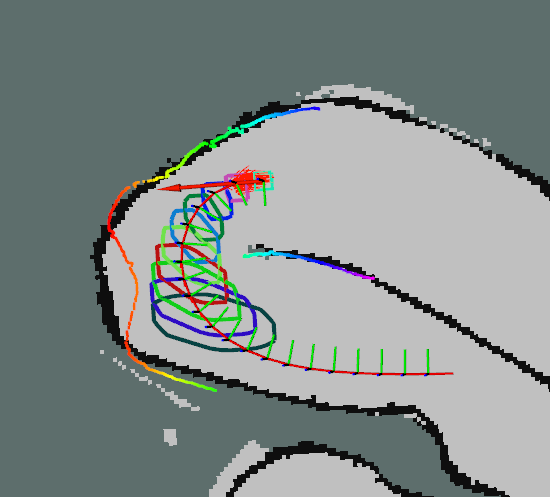
\includegraphics[width=.65\textwidth]{screenshots/FinalTopCorner.png}
    \caption{Zonotope projections from a 10-step reachability problem computed in realtime (multicolored polygons). Visualization is rendered in Rviz and shows the rasterized map in the background, overlayed by LIDAR scan data (multicolored points), MPCC trajectory (red line), and vehicle position/heading (red arrows). }
    \label{fig:my_label}
\end{figure}

We use a simple 3 variable kinematic model for the car:
\begin{equation}
\dot{x} = v \cos{\psi + d},~\dot{y} = v \sin{\psi + d},~\dot{\psi} = v \frac{1}{L} \sin(d)
\end{equation}

Define the state vector, $S= [x, y, \psi]$, and the input vector  $U = [v, d]$.
The state variable $\psi$ is the current yaw of the vehicle. The input variable $d$ is the steering angle in the vehicle's frame. The constant $L=.32$ is the wheel length of the vehicle in meters. 
An on-board Model Predictive Contouring Control  (MPCC) algorithm provides a sequence of optimal inputs for the next $N$ steps, $U_1,...,U_N$, and the corresponding predicted state trajectory is $S_1,...,S_N$. 
The non-linear kinematics are linearized around each $(S_t,U_t)$, thus obtaining the matrices $A_t,B_t$, and the linearized dynamics at step $t$ are then 
$$S_{t+1} = S_t \cdot A_t + U_t \cdot B$$
A tuning parameter $\alpha$ is introduced to scale the steering angle prior to evaluation of the Jacobian Matrices 
$$\bar{S}_t = [\bar{x}, \bar{y}, \alpha\cdot\bar{\psi}]$$
This parameter was added to address the problem of over or under steering in the linearized kinematics and was tuned experimentally to $\alpha=.5$ 


\section{Parallelizing Reachability}
Initial profiling of QuickZono using pycallgraph and cProfile revealed the large portion of computation time was spent projecting from n-dimensional zonotopes onto the useful 2-dimensional polygons which can be used to analyze safety parameters in the lower dimensional agent environment. So, this projection step was chosen as the most impactful target for parallelization. The projection was particularly well suited for this because the algorithm depends only on the target zonotope and thus is trivial to parallelize across all outputed zonotopes on the CPU.

GPU parallelization using CUDA was then written without modifying the underlying algorithm for the most time intensive function in QuickZono which is called recursively in the projection algorithm. A rudimentary strategy for parallelization was applied which directly translated the iterative CPU code into a single CUDA Kernel \ref{HybridComp}. While this section was the most time consuming piece of code, synchronous iteration was not completely avoided for the zonotope projection. Convex Hull computation was not moved to the GPU, resulting in additional copies between the host and the device to occur for each iteration of the synchronous loop. Effort was taken to minimize the number of memory copies to and from the GPU and compute resources were dynamically allocated depending on the number of vertices being considered in that particular convex hull as well as the dimension of the reachability problem. This implementation method of rewriting the code directly as one CUDA kernel abuses GPU thread abstractions to simplify translation. However, CUDA blocks (of threads) suffer from a constrained scalability compared to CUDA grids (of blocks) due to the memory layout on Nvidia GPUs. So, while we used shared memory to speed communication between threads within each block we also sacrificed the parallelism afforded by much larger grid sizes in this implementation.

\begin{figure}[t]
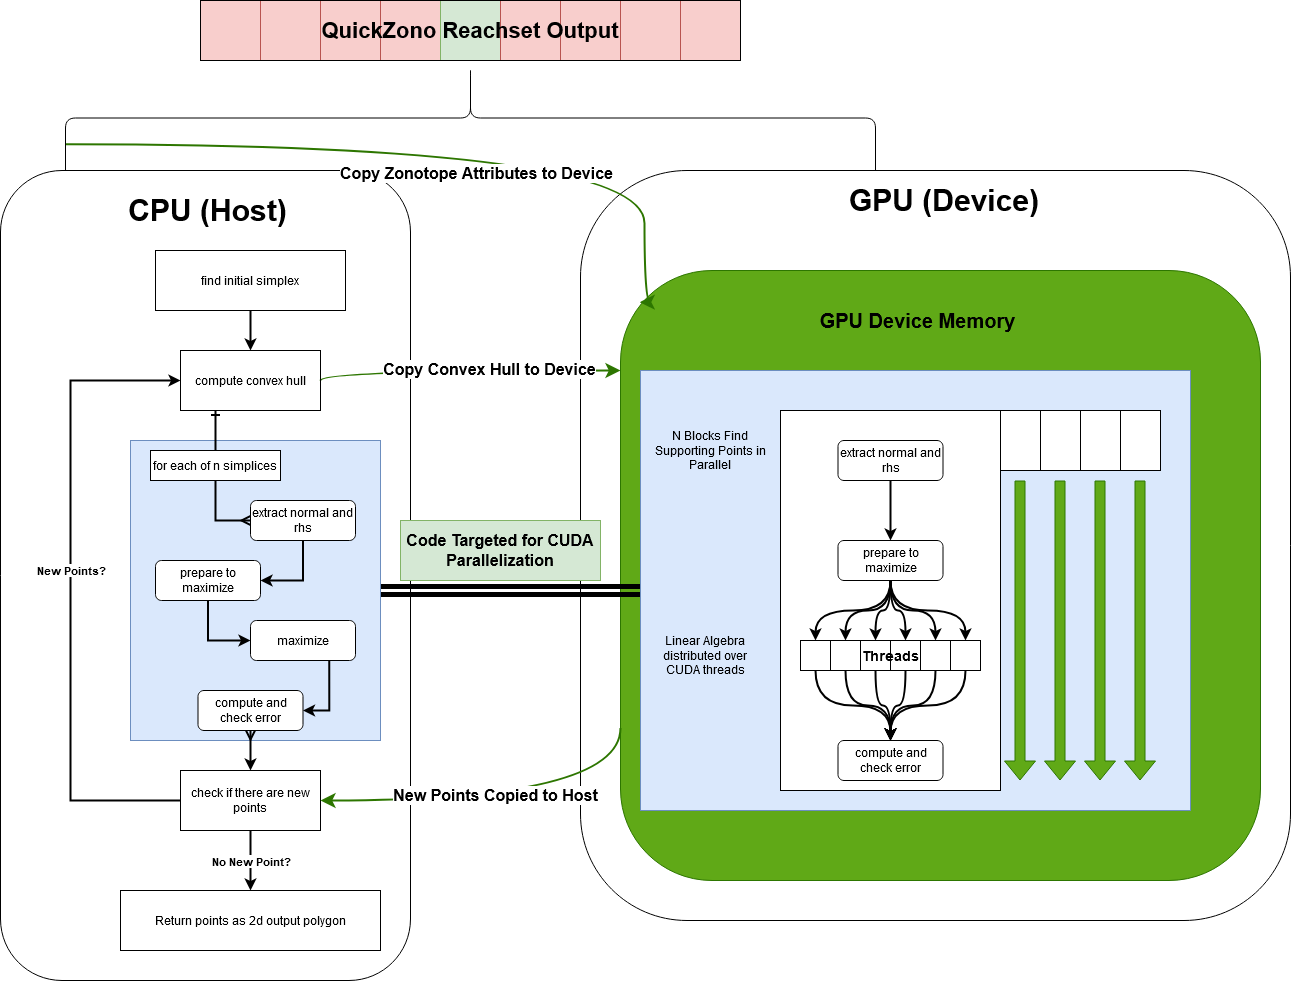
\includegraphics[width=\textwidth]{QZ_HYBRID_COMPUTATION.png}
\caption{The QZ\_HYBRID runtime mode implements a CPU/GPU hybrid computation model. Synchronous nested loops are translated to asynchronous grids of CUDA blocks in 2 dimensions. Matrix functions are distributed across 3 dimensions of threads within each block. The light blue blocks on the host and device perform analogous computations but, when executed on the GPU, as in QZ\_HYBRID, the work is distributed across hundreds of worker threads.} \label{HybridComp}
\end{figure}
\section{Experimental Setup}


\subsection{Runtime Modes}
We compare three ways of distributing the code between the CPU cores and the GPU cores:

%\subsubsection{HYLAA} \newline The original hybrid reachability tool [cite].
%\vspace*{-10pt}
\textbf{Quickzono Single Core} [QZ\_CPU]: A simplified subset of HYLAA code with succinct wrappers. 

\textbf{Quickzono Multiple Core} [QZ\_MP]: Quickzono code with a trivial CPU-based multiprocessing model \newline applied to the projection step. 

\textbf{Quickzono GPU Hybrid} [QZ\_HYBRID]: Hybrid GPU/CPU implementation, with the most taxing part of the projection algorithm moved onto the GPU device. 


\subsection{Profiling Reachability Within the Stack}

In \textit{offline} profiling, reachability is computed as the sole program running on the system. 

In \textit{online} profiling, reachability is computed as part of a ROS network running physical control nodes (controller input, motor and servo control, etc.), a GPU-based particle filter node for localization, a model predictive control node, and various other supporting nodes. 
Before beginning the profiling, the vehicle is placed into the test track, localized and configured to autonomously drive the track until profiling is complete. 
%The reachability node is implemented as a wrapper for the various reachability modes described above and records call timings for the same function, executing as quickly as possible. 
The online profiler is configured to automatically switch between number of reachability steps. Between runtime modes, the reachability node is  This occurs for the same parameters as in offline profiling, except that only those configurations executing at least 4hz ($\lt$250ms per trial) are considered. %Full HYLAA is not tested in this profiling due to slow performance.

\paragraph{Performance Characteristics}
Evaluating an embedded reachabiltiy algorithm is done using the following metrics: 
1) first of course is correctness: namely that the computed set is indeed a reachset for the dynamics. To validate correctness, we used HYLAA output as the ground truth.

2) Next is runtime: running a safety algorithm is only effective when there is a low latency between consecutive executions. If this criterion is not met, safety analysis could be out of date when the agent is developing a response.
A dedicated testing script executes each of the runtime modes for 200 trials, for $N$ reachability steps where $N$ is between 4 and 24. 
We report average and standard deviation of runtimes over the 200 trials.
%HYLAA is only tested over 5 trials due to slow performance. 
The script outputs timing data excluding any one-off setup and configuration code.

3) Third is scalability with the number $N$ of reachability time steps. 

4) Finally is runtime variability: The consistency of the tool's runtime is paramount for autonomous systems. 
Runtime spikes at the wrong time could create dangerous situations for the agent. 
Runtime variability is measured by runtime standard deviation, and we also report the  95\% confidence intervals around the mean assuming normally distributed variation in runtimes.


\section{Results}

\begin{figure}[t]
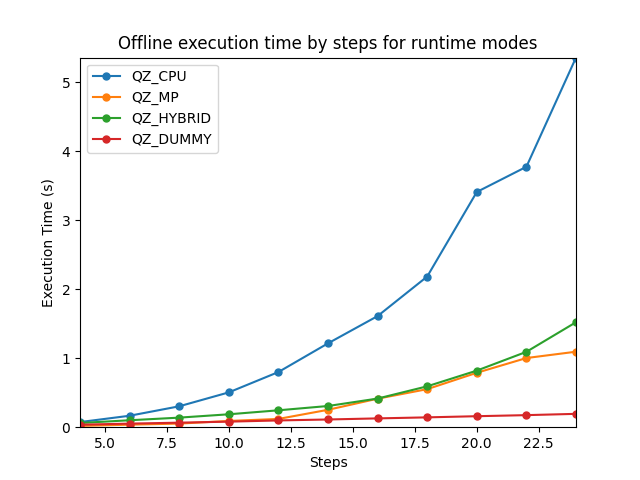
\includegraphics[width=.5\textwidth]{profiler_out/offline_avg_unified.png}
\caption{Average Offline trial execution times for all runtime modes.} \label{offline_avg}
\end{figure}

\begin{figure}[t]
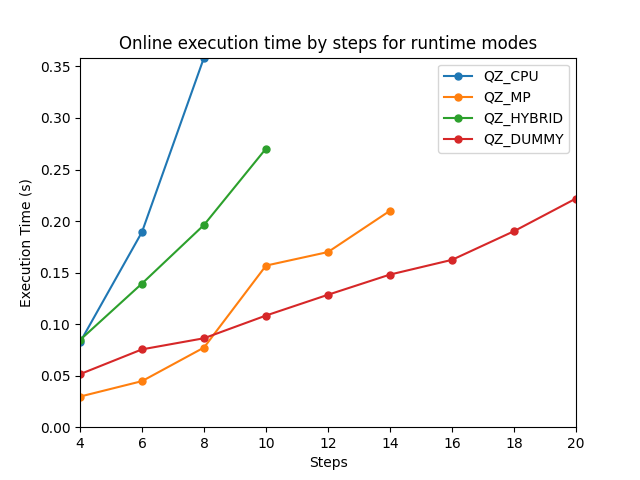
\includegraphics[width=.5\textwidth]{profiler_out/online_avg_unified.png}
\caption{Average Online trial execution times for all runtime modes.} \label{online_avg}
\end{figure}
\begin{figure}[t]
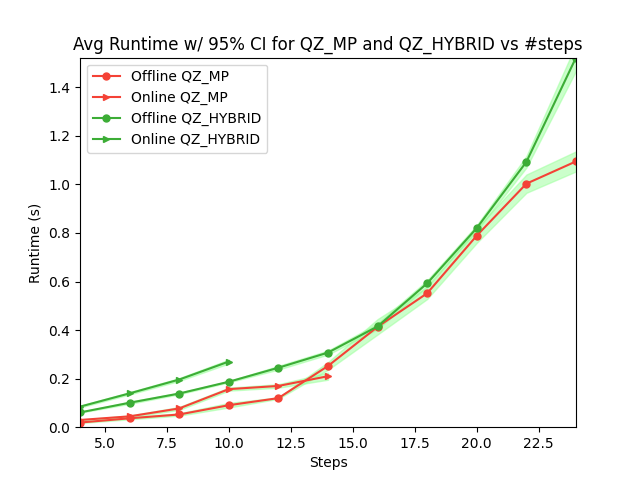
\includegraphics[width=.5\textwidth]{profiler_out/avg_mp_hybrid_CI.png}
\caption{Comparison between Multiprocessing and Hybridized online and offline runtimes.} \label{mp_hybrid_ci}
\end{figure}

\subsection{Discussion}

Realtime reachability performance at 4hz or greater was achieved for both QZ\_MP and QZ\_HYBRID runtime modes. This represents a significant performance improvement over QZ\_CPU for both methods of parallelization \ref{offline_avg}. We achieved an improvement in runtime based on straightforward techniques for GPU Parallelization with Nvidia CUDA. This is important because GPU resources are more powerful than CPU resources if they can be properly utilized. Process based parallelization on in QZ\_MP showed improvement larger than \%60 at 10 time steps over QZ\_CPU. But the multiprocessing attempt strained four CPU cores which may be better utilized in other critical applications. Notably, 

Online modes had generally higher runtimes (slower) than offline modes for all steps across all rutnime modes (show pvalues??). This is sensible due to increased CPU load in online mode from SLAM + MPCC algorithms. \ref{online_avg} Despite improved scalability of QZ\_HYBRID vs QZ\_CPU \ref{offline_avg} the two runtime modes have comparable timings at the lowest number of reachability steps. The overhead of making CUDA device calls for initializing GPU memory in QZ\_HYBRID may explain this discrepancy.

Comparison of QZ\_MP and QZ\_HYBRID shows a much larger 95\% confidence interval for CPU\_MP  in the offline mode. This is unexpected given anticipated variation introduced by calling CUDA functions. \ref{mp_hybrid_ci} While online execution of QZ\_HYBRID is slower than QZ\_MP, offline timings are very similar for the two modes between 14 and 22 steps. So, performance of QZ\_HYBRID is comparable to that of QZ\_MP at these configurations despite only utilizing a single CPU core. This indicates a potential for reduced CPU load without sacrificing reachability performance through only naive parallelization techniques.


%
% ---- Bibliography ----
%
% BibTeX users should specify bibliography style 'splncs04'.
% References will then be sorted and formatted in the correct style.
%
\bibliographystyle{splncs04}
\bibliography{bibliography}
%
%
\end{document}
